\documentclass{article}
\usepackage[utf8]{inputenc}
\usepackage{graphicx}
\usepackage{subcaption}
\usepackage{geometry}
\geometry{left=38mm,top=30mm,bottom=30mm,right=25mm}

\begin{document}
\begin{titlepage}
\newcommand{\HRule}{\rule{\linewidth}{0.5mm}}

\center
\textsc{\LARGE \textbf{Open Science Project}}\\[1 cm]

\textsc{\Large Windrose Python Package}\\[0.5 cm]

\textsc{\large Jacob Newman (201528601)}\\[0.5 cm]





\vfill\vfill\vfill
{\large\today}
\vfill

\end{titlepage}


\section{Introduction}\label{Introduction}
Great strives to better understand and display historical climatological data have been made in the past decade due to growing concerns over climate change among other things. One climatological data set 
that has a diverse range of importance when addressing these problems is wind data. Changes in major wind patterns, such as increases in the power of wind systems over time, can be used as a gauge to 
measure how the strength of storms is changing due to climate change (Mendelsohn et al. 2012). Another application of study of wind data, in particular directional wind data, is designing wind power 
farms (Cetinay, Kuipers, and Guven, 2016) for a source of clean, renewable energy. For optimal placement of wind turbines, promenent wind directions and the associated wind speeds need to be plotted and 
analyzed. Other applications of studying wind data include mapping air pollution sources (Adams and Kanaroglou, 2016) and knowledge of dominate wind directions at airports, important information for 
pilots and air traffic controllers (Bellasio, 2014).
\\
\indent Here we will look at the last of the applications in connection to airports in Newfoundland and Labrador. Wind speed and directional data are collected at each airport through out the province, 
making data access relatively simple. A Python based wind data visulization package Windrose (Roubeyrie and Celles, 2018) will be employed to show several variations of polar diagrams used to plot each 
airport's respective wind data. Although we propose the purpose of this study to be that of knowledge gathering for pilots and air traffic controllers, a broad connection to the potential for wind 
energy production in the province of Newfoundland and Labrador (a long discussed topic) can be made. We a merely limited by the availablity of data to fully engage in the study of wind power potential. 
\\
\indent The remainder of this report is structed as follows, in section (\ref{Data_access}) we discuess data access and collection, in section (\ref{Wind_data_visualization}) we introduce the Windrose  
package and show multiple visualizations of direction wind data for a user-defined airport (see README), finally in section (\ref{Discussion_and_conclusions}) we breifly discuss and conclude on some key 
points.      

\section{Methodology}\label{Methodology}

\subsection{Data Access}\label{Data_access}
The README file should be consluted for prelimnanry data access information and for instructions on how to call data from a particular airport. Here we talk about where the data is from and how it is 
collected. All the data (fithteen sets) available from the windData repository was accessed through the Canadian Climate Data Accessibility Portal (CCDAP). The CCDAP is a public data query platform which 
holds Canadian historical climate data collected and maintained by Environment and Climate Change Canada. CCDAP was made at the Water Security and Climate Change Lab (WSCC) at Concordia University. As 
mentioned above, each data set was collected at an airport in Newfoundland and Labrador over some range of time (given in data set name). The data has been stripped to only include data/time, wind speed 
and wind direction information; full data sets for each locality include multiple addtional weather measures such as temperature and visiablity. The decision to only include wind data in this report (as 
other data, visiablity in particular, is also important information for air travel) was for two main reasons, firstly, the CCDAP limits the size of data sets and thus including additional weather 
measurements would restricted the range of time of each data set subsequently degraded the historical aspect of the information gather by this study. Secondy, the Windrose package currently provides no 
mechinism for analizing weather data other then wind data.
\\
\indent Each data set was collected by an aviation weather station. Since the age range of all the data is quite broad, no one system was used to collected each data set. We will therefore breifly 
discuss a commonly used aviation weather station, the Automated Weather Observtion System (AWOS) shown in figure (\ref{AWOS}). AWOS is a core component of NAV Canada's weather monitoring system with over 
100 systems in place across the country. Each system is installed on the airfield and collects weather data (e.g. wind speed and direction) continously, in real-time and sends the information directly 
to the airport and pilots. This weather data is then stored and accessed via public portals such as CCDAP for a varity of studies such as this one. 

\begin{figure}[h!]
\centering
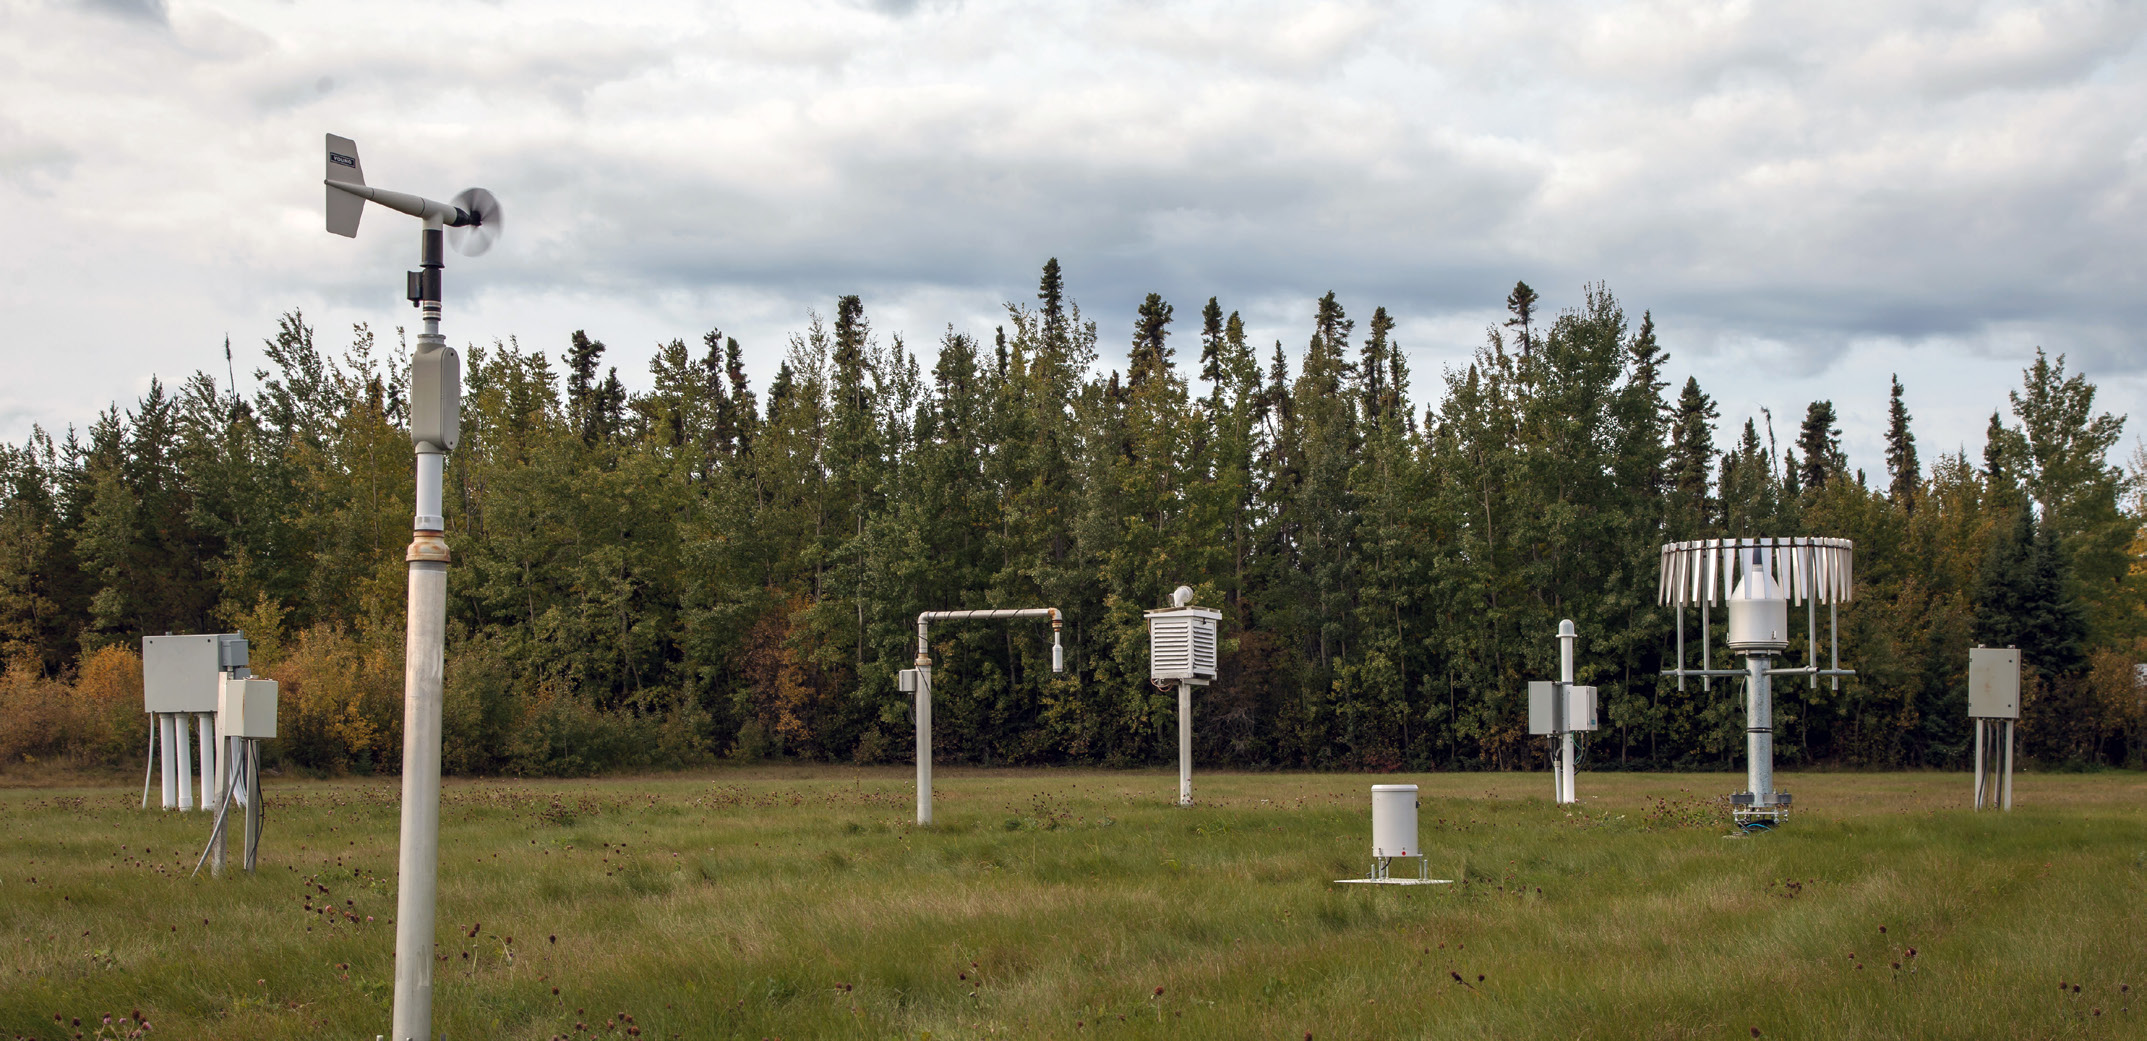
\includegraphics[width=10cm]{Images/AWOS.jpg}
\label{AWOS}
\caption{Automated Weather Observation System (AWOS) used to monitor weather at many airports throughout Canada. Older data sets or data sets from remote areas would have been collected on a similar, 
less-advanced weather station.}
\end{figure}

\subsection{Wind Data Visualization}\label{Wind_data_visualization}

The Windrose package is a graphic tool used to give a view of how wind speed and direction are typically distributed at a particular location (Roubeyrie and Cellers, 2018). The package is backend my 
Matplotlib to produce multiple polar (rose) diagrams for a given data set. These Windrose diagrams can subsquently be used in applications mentioned in section (\ref{Introduction), among others. When 
these diagrams are tied with positional digrams, such as the one seen in figure (\ref{location}) showing the location of the data presented in this report, links can be made between environmental aspect 
(wind tunnel effects, proximity to oceans, etc.) and the preferred wind directions.

\begin{figure}[h!]                                                                                                                                                                                                 
\centering                                                                                                                                                                                                         
\includegraphics[width=10 cm]{location.pdf}                                                                                                                                                                        
\label{location}                                                                                                                                                                                                   
\caption{Map of Newfoundland and Labrador annoted by location of wind data collection (yellow star).}                                                                                                              
\end{figure} 
  
\begin{figure}[h!]
\centering
\includegraphics[width=10cm]{bar.pdf}
\caption{Directional wind data from user-defined Newfoundland and Labrador airport plotted on a bar polar diagram from the Windrose Python package.}
\label{bar_windrose}
\end{figure}

\begin{figure}[h!]
\centering
\includegraphics[width=10cm]{box.pdf}
\caption{Directional wind data from user-defined Newfoundland and Labrador airport plotted on a box polar diagram from the Windrose Python package.}
\label{box}
\end{figure}

\begin{figure}[h!]
\centering
\includegraphics[width=10cm]{contour.pdf}
\caption{Directional wind data from user-defined Newfoundland and Labrador airport plotted on a contour polar diagram from the Windrose Python package.}
\label{contour_windrose}
\end{figure}

\begin{figure}[h!]
\centering
\includegraphics[width=10cm]{contourf.pdf}
\caption{Directional wind data from user-defined Newfoundland and Labrador airport plotted on a filled contour polar diagram from the Windrose Python package.}
\label{contourf_windrose}
\end{figure}

\section{Disscusion and Conclusions}\label{Disscusion_and_conclusions}

\end{document}
